\chapter{Medical Imaging and Image Segmentation}
%

The first steps in image-based modeling and simulation involve image acquisition, image processing, and image segmentation. Several techniques are available to produce three-dimensional image data of an anatomical region of interest and are reviewed herein. State-of-the art image processing and image segmentation approaches are summarized in this section as well.

%%%%%%%%%%%%%%%%%%%%%%%%%%%%%%%%%%%%%%%%%%%%%%%
%%%%%%%%%%%%%%%%%%%%%%%%%%%%%%%%%%%%%%%%%%%%%%%
\section{Imaging Approaches}
\label{Imaging Approaches}

Medical imaging is the process of generating discrete image representations of biological tissues. Of the many imaging modalities found in clinical and research settings, the most prevalent are magnetic resonance imaging (MRI) and x-ray computed tomography (CT). Both approaches are \textit{tomographic} in that they produce a series of two-dimensional images representing thin slices through the region, that are subsequently combined to produce a three-dimensional volume representation \cite{larobina_murino_2014}. The data measured during acquisition are different for each modality, and thus a particular technique may be more desirable depending on the use case. Several other imaging techniques exist - some of which provide more information than what MRI and CT provide - and are briefly discussed in this section as well.

\subsection{Magnetic Resonance Imaging}
\label{Magnetic Resonance Imaging}



\subsection{X-Ray Computed Tomography}
\label{X-Ray Computed Tomography}

houndsfield units

\subsection{Additional Imaging Modalities}
\label{Other Imaging Modalities}

\subsection{Data Format}
\label{Data Format-IMG}
Medical images are typically stored in 

%%%%%%%%%%%%%%%%%%%%%%%%%%%%%%%%%%%%%%%%%%%%%%%
%%%%%%%%%%%%%%%%%%%%%%%%%%%%%%%%%%%%%%%%%%%%%%%
\section{Image Segmentation Approaches}
\label{Image Segmentation Approaches}

Arguably the most challenging task in the workflow is the subsequent image processing and \textit{segmenting} of the image of interest.

\subsection{Thresholding Methods}
\label{Thresholding Methods}

\subsection{Region-Growing Methods}
\label{Region-Growing Methods}

\subsection{Neural Networks}
\label{Neural Networks}

\subsection{Manual Methods}
\label{Manual Methods}

\begin{figure}[ht]
\centering
\subfigure[]{%
		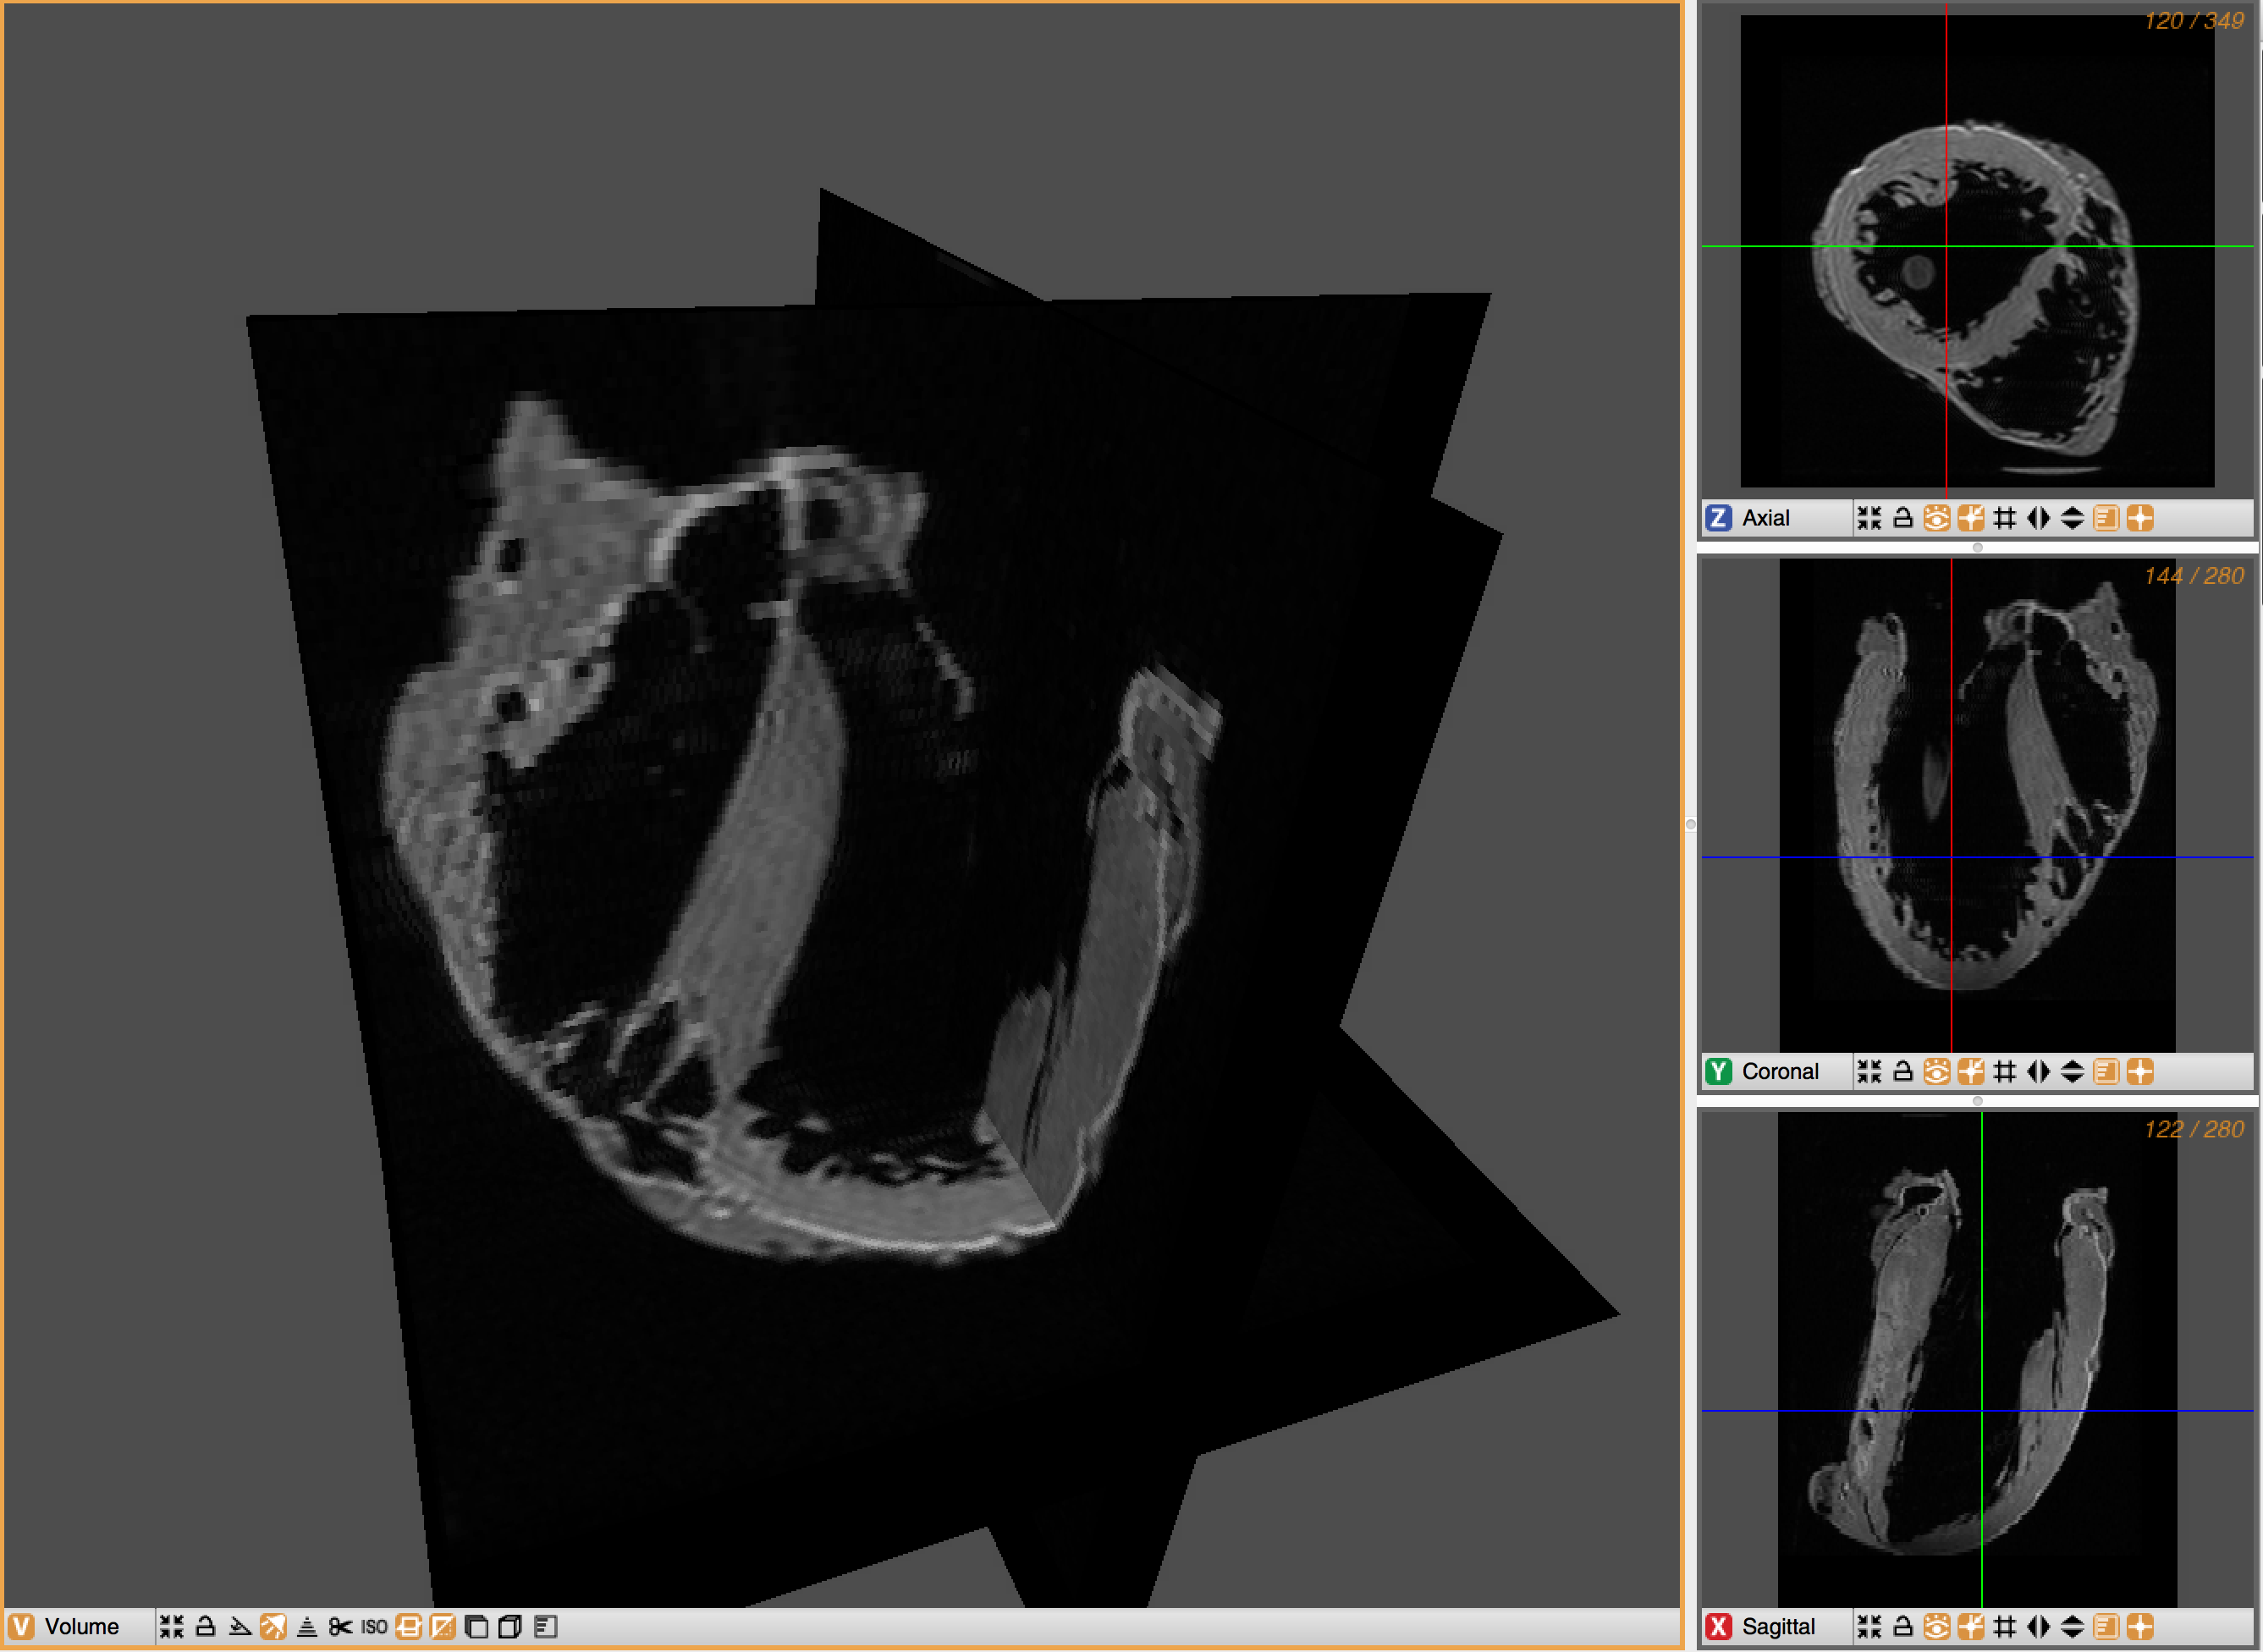
\includegraphics[scale=0.165]{media/1-seg3d/1-raw.png}
\label{fig:seg1}}
\subfigure[]{%
		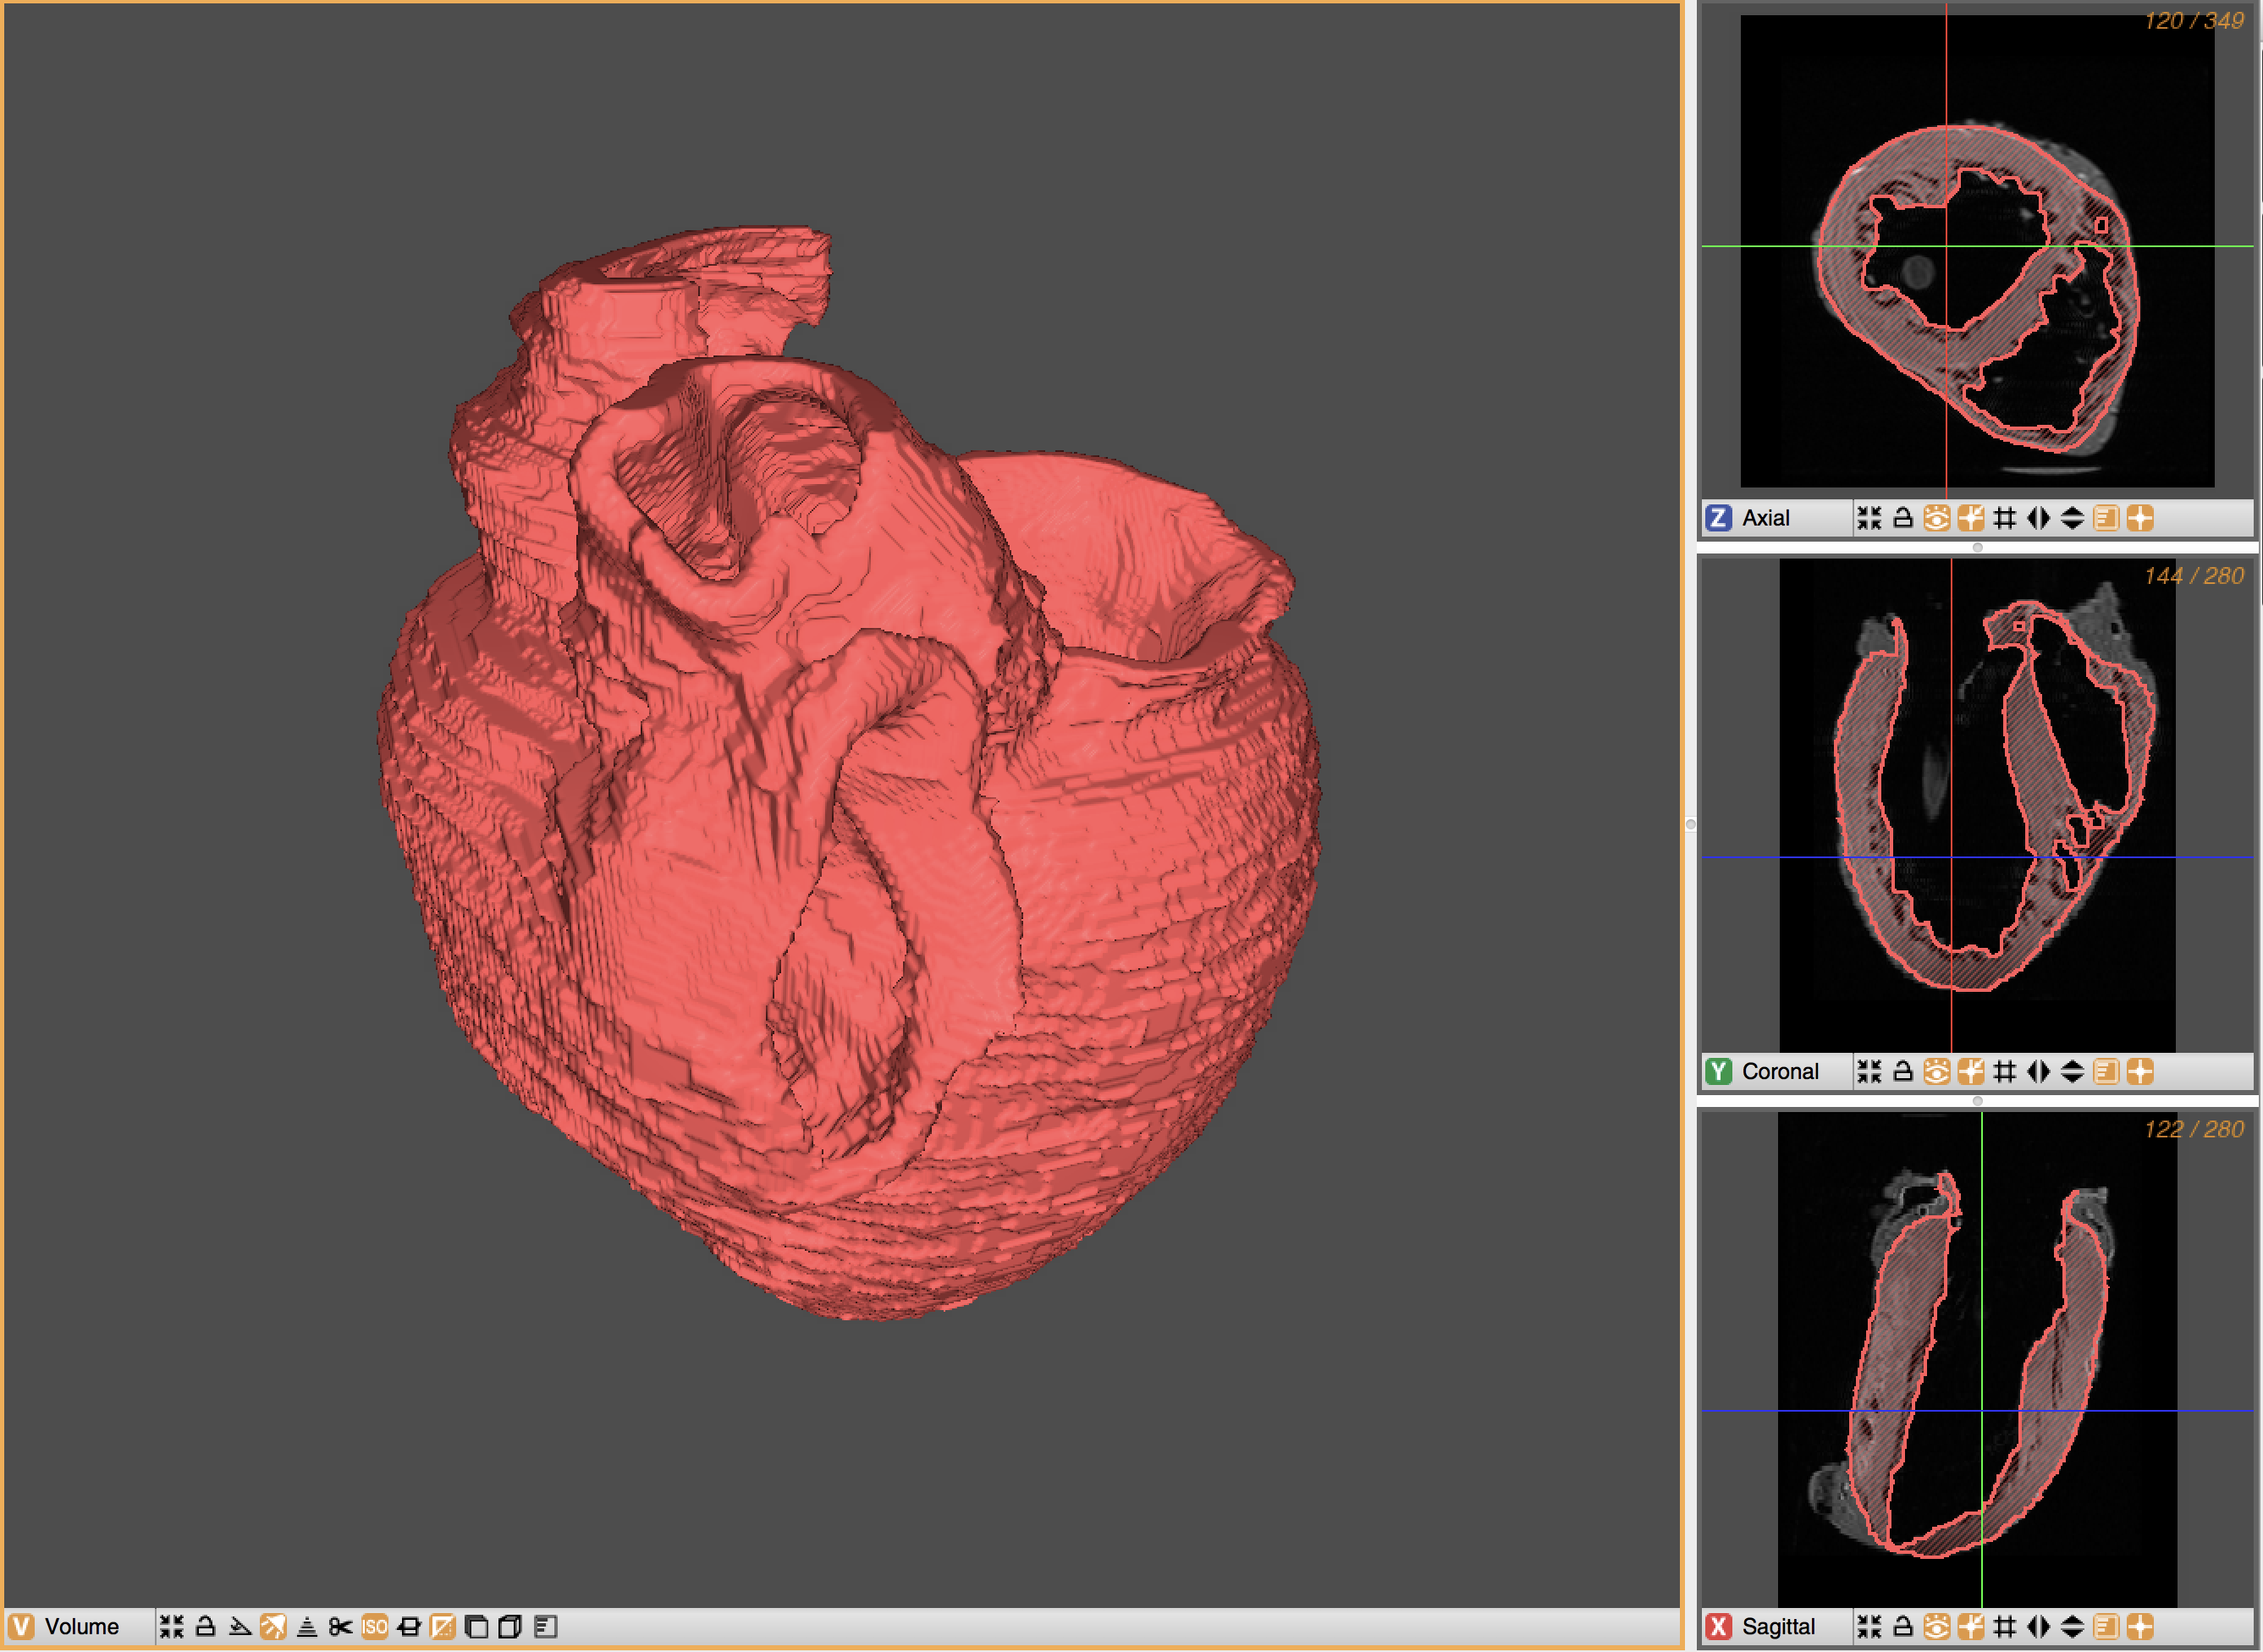
\includegraphics[scale=0.165]{media/1-seg3d/2-seg.png}
\label{fig:seg2}}
%
\caption{(a) MRI of \textit{ex-vivo} human heart, and (b) resulting segmented image mask}
\label{fig:seg}
\end{figure}